\pdfminorversion=4
\documentclass{beamer}
\usepackage[T1]{fontenc}
\usepackage[ngerman]{babel}
\usepackage[utf8]{inputenc}
\usepackage[babel,german=quotes]{csquotes}
\usepackage{amsmath,amsfonts,amssymb}
\usepackage{hyperref}
\usepackage{lmodern}
\usepackage{microtype}

\usetheme{fau-4-3}

\usepackage[sort&compress,comma,super,square]{natbib}
%\bibliographystyle{apalike} % Or your specific bibliographystyle
\bibliographystyle{unsrtdin}
%\bibliographystyle{gerplain}

\newcommand{\todo}[1]{\textbf{\color{red}{TODO: #1}}}


\title{cowbusconfig – Ansatz zur dezentralen Konfiguration von Gebäudeautomation}
\author[P. Kanzler, M. Zapf]{Patrick\,Kanzler \and Michael\,Zapf}
\date{23.09.2015}

% space between items
\newcommand{\customitemsep}{7pt}
\newcommand{\customitemsepsub}{2pt}

\begin{document}
\frame{\titlepage}

%\section{cowbusconfig – Ansatz zur dezentralen Konfiguration von Gebaueudeautomation}
\begin{frame}
	\frametitle{Der Traum von der schönen neuen Welt}

	\begin{itemize} \setlength{\itemsep}{\customitemsep}
		\item \todo{schön darstellen, vielleicht mit Bildern, momentan nur Stichpunkte}
		\item Haus der Zukunft
		\item z.B. Beleuchtung folgt intelligent durch das Haus
        \item scheitert bisher: komplizierte Einrichtung, teure Komponenten, keine Standards
	\end{itemize}
\end{frame}

\begin{frame}
	\frametitle{Ansätze}
    \begin{columns}[c]
        \column[c]{10cm}
            \textbf{EIB/KNX} \cite{knx-prod}
            \begin{itemize} \setlength{\itemsep}{\customitemsep}
                \item etabliertes System
                \item viele Produkte auf dem Markt
                    \vspace*{0.5cm}
                \item \textcolor{red}{aufwändige (Neu-)Einrichtung}
            \end{itemize}
        \column{10cm}
            \textbf{Skriptserver} \\
            {\fontsize{15pt}{18pt} \selectfont (z.B. nach Haenselmann et al. \cite{haenselmann2007skriptbasierte})}
            \begin{itemize} \setlength{\itemsep}{\customitemsep}
                \item zentrale Stelle mit Schaltregeln
                \item Skripte jederzeit anpassbar
                    \vspace*{0.5cm}
                \item \textcolor{red}{\enquote{Single Point of Failure}}
            \end{itemize}
    \end{columns}
\end{frame}

\begin{frame}
    \frametitle{Ziele und Ideen}

    \begin{itemize} \setlength{\itemsep}{\customitemsep}
        \item dezentrale Organisation
        \item komfortable Konfiguration, nicht jeden Knoten \enquote{anfassen} müssen
            \begin{itemize} \setlength{\itemsep}{\customitemsepsub}
                \item z.B. Webbrowser vom Notebook/Tablet aus
                \item[$\Rightarrow$] Gateway vom LAN/WLAN ins Sensornetz benötigt
            \end{itemize}

        \item einfach nachvollziehbare Schaltregeln
        \item typische Anforderungen an Energieversorgung beachten
            \begin{itemize} \setlength{\itemsep}{\customitemsepsub}
                \item oft: Aktoren besitzen stabile Stromversorgung
                \item Sensoren eher klein, flexibel, sparsam
                \item[$\Rightarrow$] Aufteilung in \enquote{dumme} Sensoren und \enquote{intelligente} Aktoren
                \item[$\Rightarrow$] eigentliche Entscheidungs- bzw. Schaltlogik{dumme} in Aktoren
            \end{itemize}
    \end{itemize}
\end{frame}

\begin{frame}
    \frametitle{Regeln}

    \begin{itemize} \setlength{\itemsep}{\customitemsep}
        \item Annahme: (virtuelle) Knoten durch eindeutige Adresse identifizierbar
        \item Annahme: Sensorpaket enthält nur einen Wert, Bedeutung bekannt
        \item[ ] \vspace*{0.5cm}
            \pause
        \item Quelladresse
        \item Typ des Vergleichs ($<$, $>$, ==, !=, $<>$)
        \item Grenzwert(e)
        \item auszuführende Aktion
            \begin{itemize} \setlength{\itemsep}{\customitemsep}
                \item Muss dem Aktor bekannt sein!
            \end{itemize}
    \end{itemize}
\end{frame}

\begin{frame}
    \frametitle{Konfigurationsnachrichten}

        Ziele:
            \begin{itemize} \setlength{\itemsep}{\customitemsep}
                \item Kommunikation in-band, Standort egal
                \item Konfiguration jederzeit auslesbar und änderbar
            \end{itemize}

            \pause
        \vspace*{1cm}


        3 Typen ausreichend: LIST, ADD, DELETE
            \begin{itemize} \setlength{\itemsep}{\customitemsep}
                \item \textbf{LIST} fordert alle Regeln eines Knotens an
                \item \textbf{ADD} erstellt eine neue Regel auf einem Knoten
                \item \textbf{DELETE\_ONE} löscht eine Regel auf einem Knoten
            \end{itemize}
\end{frame}

\begin{frame}
    \frametitle{Demo}
        Sensor:
        \begin{itemize} \setlength{\itemsep}{\customitemsep}
            \item cowbus-protoboard mit RIOT und einfacher Anwendung
            \item 4 Taster, Temperatursensor
        \end{itemize}
        \vspace*{0.75cm}
        \pause

        Aktor:
        \begin{itemize} \setlength{\itemsep}{\customitemsep}
            \item cowbus-protoboard mit RIOT und einfacher Anwendung
            \item RGB-LED, Piezo-Summer
        \end{itemize}
        \vspace*{0.75cm}
        \pause

        Gateway:
        \begin{itemize} \setlength{\itemsep}{\customitemsep}
            \item Raspberry Pi B
            \item Funkmodul per SPI angebunden
        \end{itemize}
        \vspace*{1cm}
\end{frame}

\section{Vielen Dank für Ihre Aufmerksamkeit!}
\section{Q\&A}

\bibliography{2015-09-cowconfig}{}

%\begin{frame}[plain]
%    \center
%    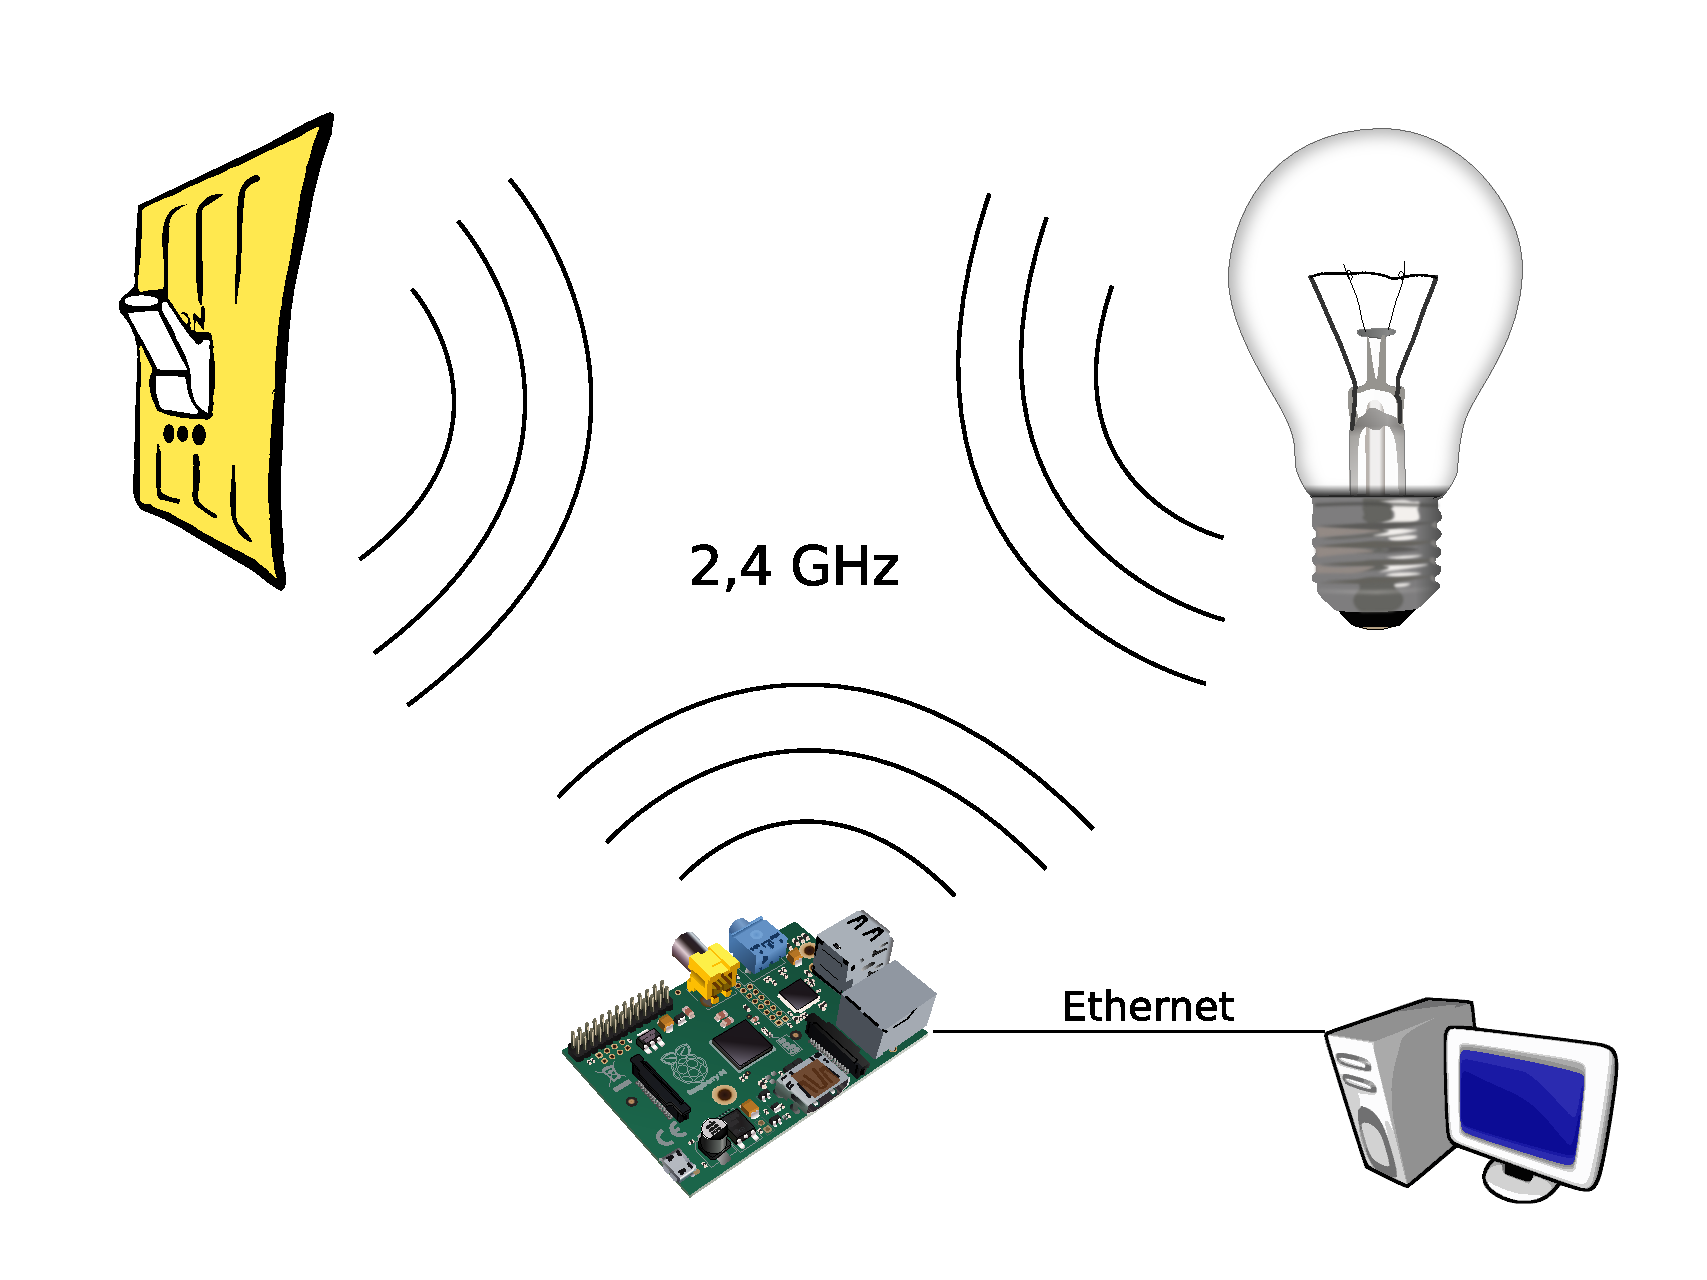
\includegraphics[scale=0.4]{img/system}
%\end{frame}


%\nocite*

\end{document}

